\documentclass{article}
\usepackage[utf8]{inputenc}
\usepackage{subfiles}
\usepackage{amsmath}
\usepackage{pgfplots}
\usepackage{textcomp}
\usepackage{csquotes}
\pgfplotsset{compat=1.13}
\pgfplotsset{width=10cm}
\pgfplotsset{holdot/.style={color=blue,fill=white,only marks,mark=*}}
\pgfplotsset{dot/.style={color=blue,fill=blue,only marks,mark=*}}
%\usepgfplotslibrary{fillbetween}

\title{Noah's Guide to Calculus}
\author{Noah Stockwell}
\date{Summer 2016}

\begin{document}

\maketitle

\vspace{2in}
\begin{center}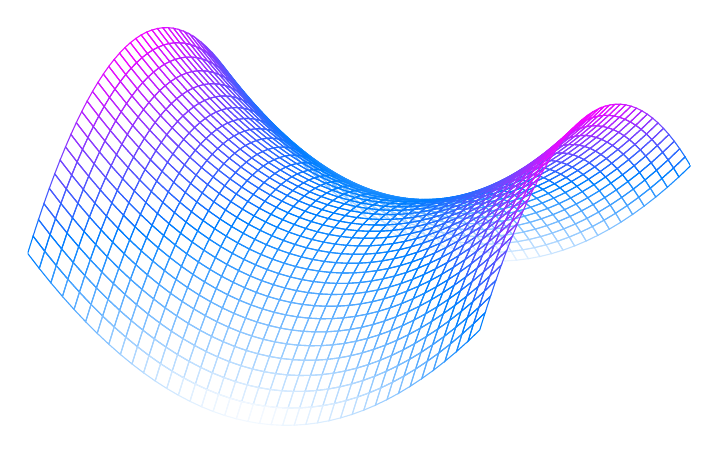
\begin{tikzpicture}\begin{axis}[hide axis,
xlabel=$x$,ylabel=$y$,colormap/cool, ]
\addplot3[domain=-3:3,mesh,samples=40]{x^2-y^2};
\end{axis}\end{tikzpicture}\end{center}
\newpage

\tableofcontents
\newpage

\section{Introduction}\subfile{sections/introduction}\newpage

\section{Limits}\subfile{sections/limits}\newpage

\section{Derivatives}\subfile{sections/derivatives}\newpage



\end{document}